\begin{frame}[t]{Ideals for Parallel Patterns}
\begin{itemize}[<+->]
  \item Applications should be expressed \textmark{independently} of the
        \textgood{execution model}.
  \vfill
  \item \textmark{Computations} should be expressed in terms of 
        \textgood{structured composable patterns}.
  \vfill
  \item \textgood{Multiple back-ends} should be offered with \textmark{simple switching}
        mechanisms.
  \vfill
  \item Interface should \textmark{integrate} seamlessly with \textgood{modern C++} and
        its standard library.
  \vfill
  \item Applications should be able to \textmark{take advantage} of \textgood{modern C++} language features.
\end{itemize}
\end{frame}

\begin{frame}[t]{C++17: Execution policies}
\begin{itemize}
  \item An \textmark{execution policy} allows to disambiguate 
        parallel algorithms overloads.
    \begin{itemize}
      \vfill
      \item \cppid{sequenced\_policy}: 
            Not parallelized.
        \begin{itemize}
          \item \cppid{std::execution::seq}.
        \end{itemize}

      \vfill
      \item \cppid{parallel\_policy}: 
            Execution can be parallelized in multiple threads.
        \begin{itemize}
          \item \cppid{std::execution::par}.
        \end{itemize}

      \vfill
      \item \cppid{parallel\_unsequenced\_policy}:
            Execution can be parallelized, vectorized, or migrated across threads.
        \begin{itemize}
          \item \cppid{std::execution::par\_unseq}.
        \end{itemize}
    \end{itemize}
\end{itemize}
\end{frame}

\begin{frame}[t,fragile]{C++17: Parallel algorithms}
\begin{itemize}
  \item Most algorithms in \cppid{<algorithm>} and \cppid{<numeric>}
        have \textmark{execution policy} based versions.
\end{itemize}

\pause
\begin{block}{SAXPY: C++17}
\begin{lstlisting}[escapechar=@]
std::transform(@{\color{red}std::execution::par}@,
  y.begin(), y.end(), x.begin(), y.begin(),
  [=](auto vx, vy) { return a * vx + vy; });
\end{lstlisting}
\end{block}

\pause
\begin{itemize}
  \item However \ldots
    \begin{itemize}
      \item No fine control knobs.
      \item Lack of task parallelism and stream parallelism.
      \item OK as an entry level to parallelism.
    \end{itemize}
\end{itemize}
\end{frame}

\begin{frame}[t]{GrPPI}
\begin{Large}
\textgood{\url{https://github.com/arcosuc3m/grppi}}
\end{Large}
\vfill\pause
\begin{itemize}
  \item \textgood{G}eneric \textgood{r}eusable \textgood{P}arallel
        \textgood{P}attern \textgood{Interface}.
    \begin{itemize}
      \item A header only library (might change).
      \item A set of execution policies.
      \item A set of type safe generic algorithms.
      \item Requires \textgood{C++14}.
      \item Apache 2.0 License.
    \end{itemize}
\end{itemize}
\end{frame}

%\begin{frame}[t]{GrPPI as a teching tool}
%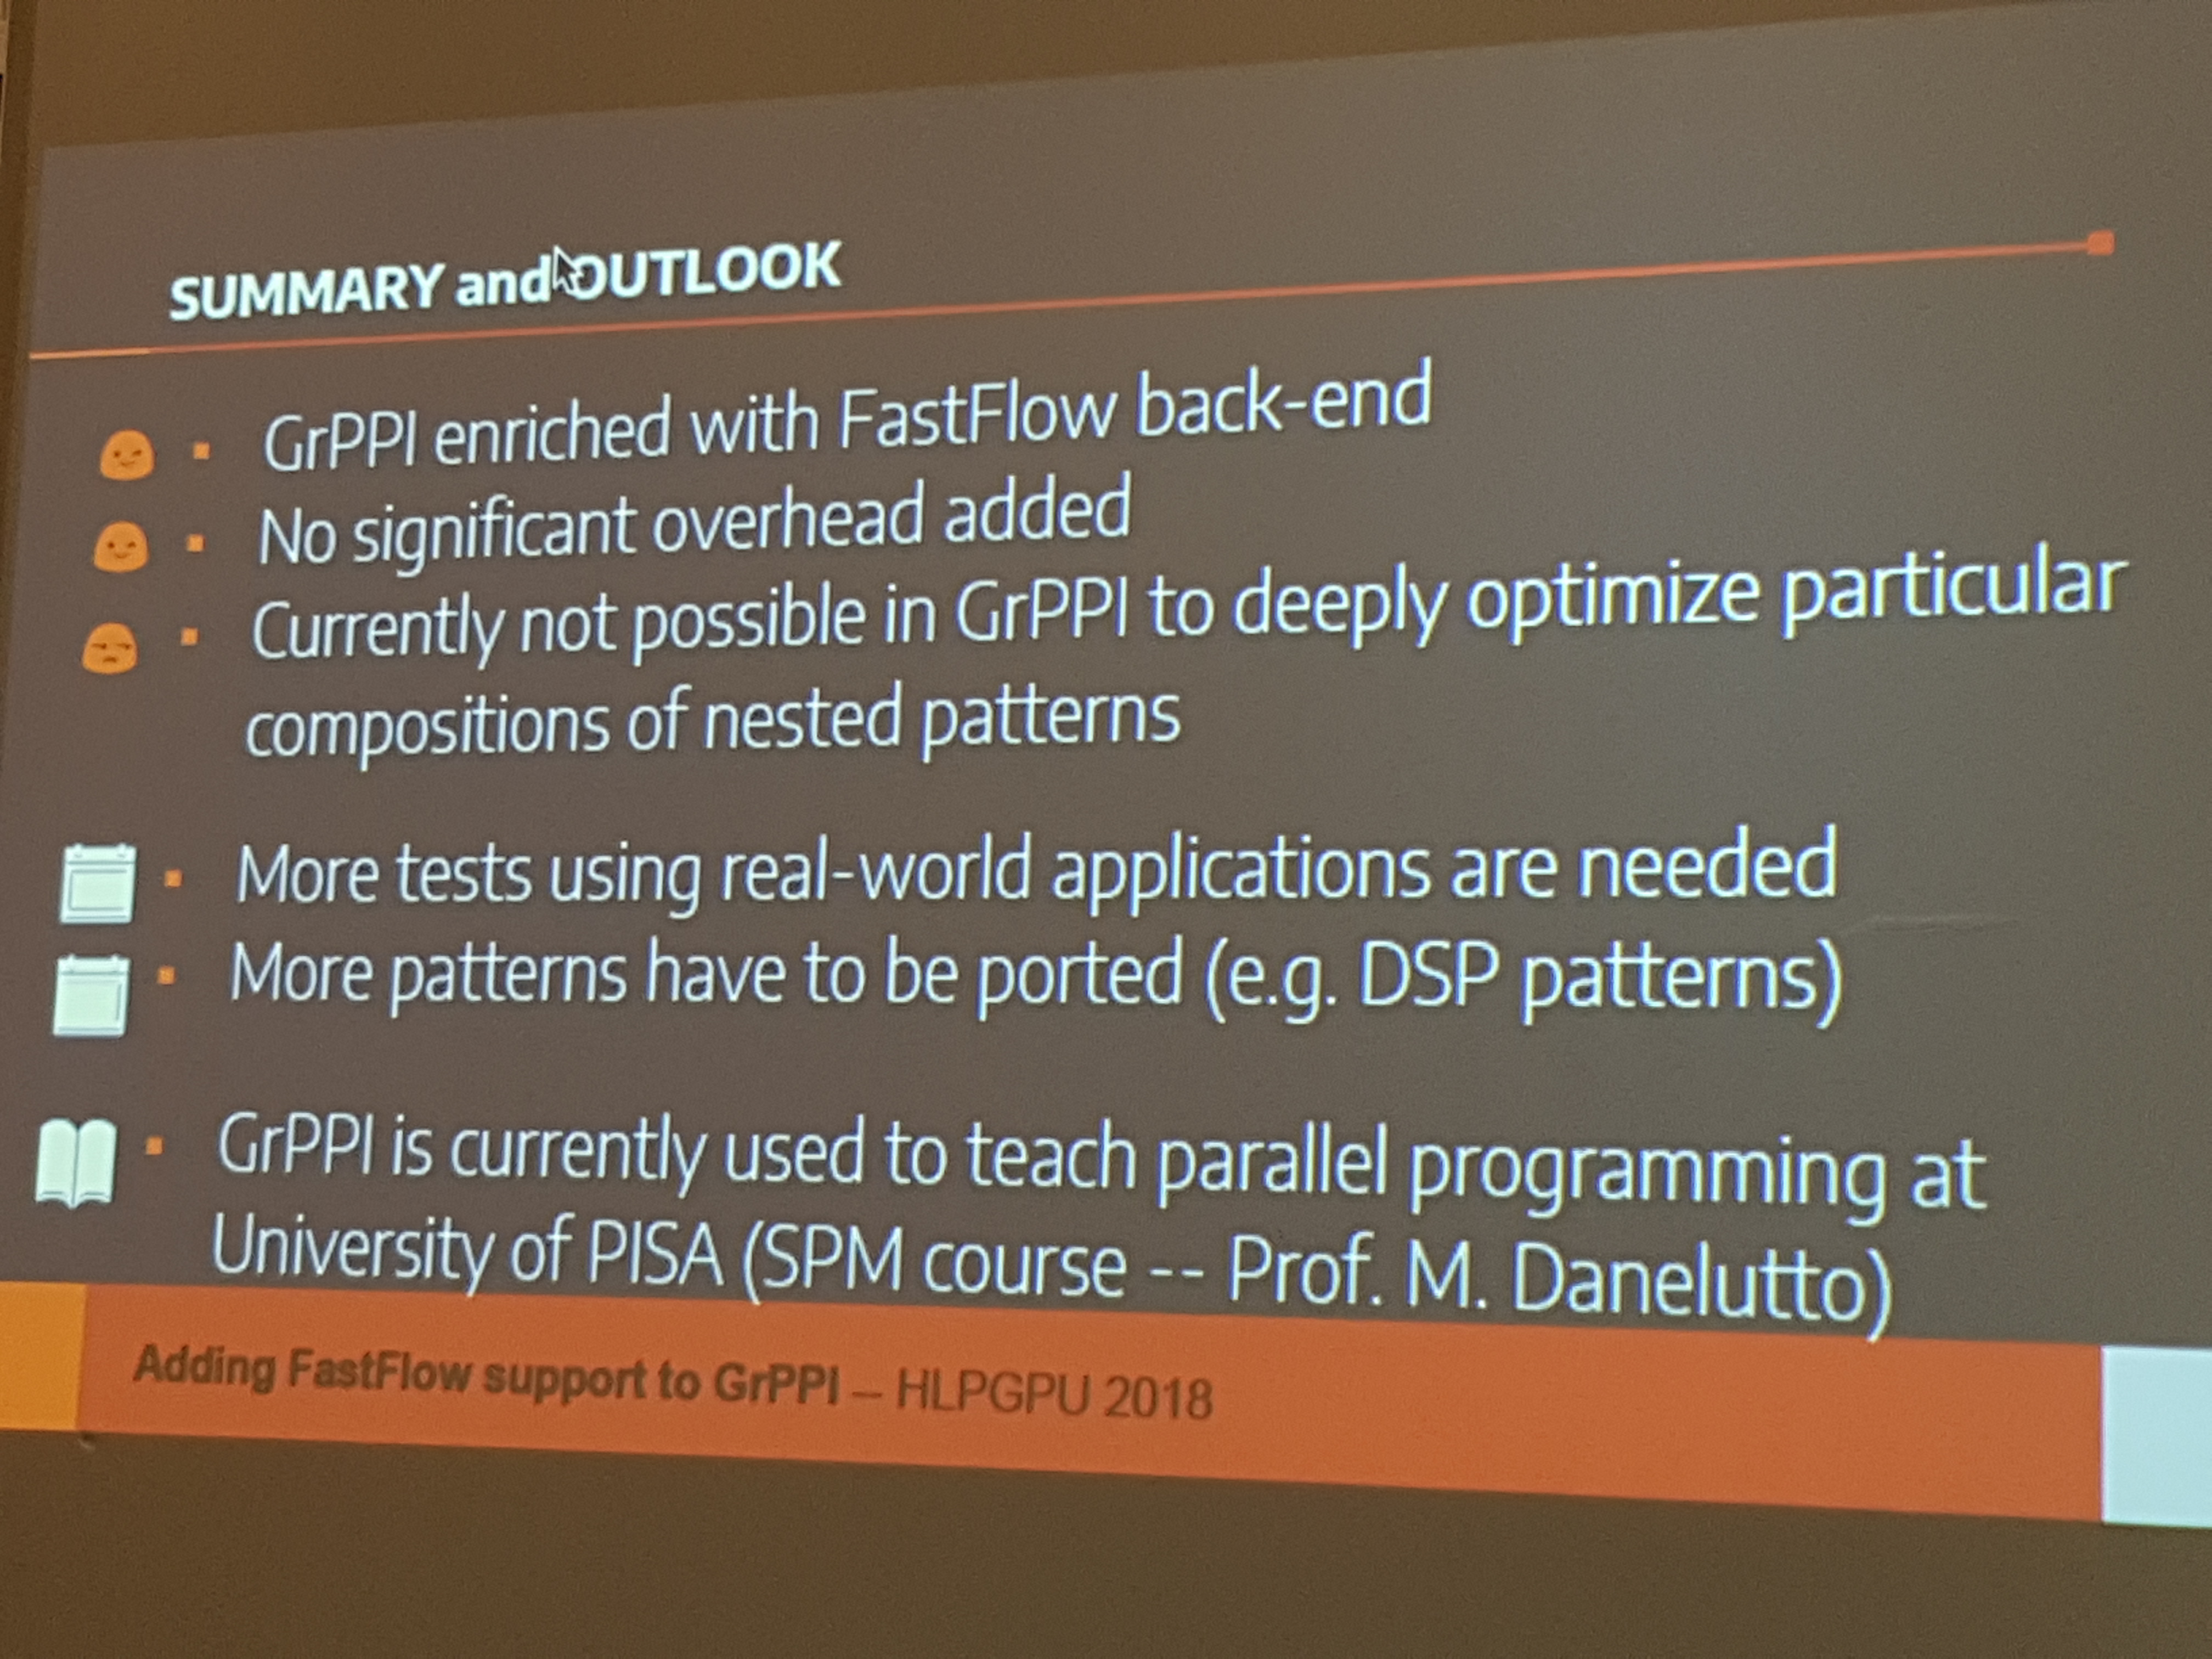
\includegraphics[width=\textwidth]{img/grppi-upi.jpg}
%\end{frame}
